%% LyX 2.1.1 created this file.  For more info, see http://www.lyx.org/.
%% Do not edit unless you really know what you are doing.
\documentclass[12pt,english]{article}
\usepackage[T1]{fontenc}
\usepackage[utf8]{inputenc}
\usepackage{geometry}
\geometry{verbose}
\setlength{\parskip}{\smallskipamount}
\setlength{\parindent}{0pt}
\usepackage{float}
\usepackage{graphicx}
\usepackage{setspace}
\usepackage[authoryear]{natbib}
\doublespacing

\makeatletter

%%%%%%%%%%%%%%%%%%%%%%%%%%%%%% LyX specific LaTeX commands.
%% Because html converters don't know tabularnewline
\providecommand{\tabularnewline}{\\}

%%%%%%%%%%%%%%%%%%%%%%%%%%%%%% Textclass specific LaTeX commands.
\usepackage{ifpri}

\makeatother

\usepackage{babel}
\begin{document}

\title{Fertility, Agricultural labour Supply and Production - Instrumental
Variable Evidence from Uganda}


\author{Bjorn Van Campenhout\division{Development Strategy and Governance Division}
\cpauthor{Bjorn Van Campenhout, International Food Policy Research Institute\\ Research Fellow, Development Strategy and Governance Division\\{b.vancampenhout@cgiar.org}}}
\maketitle
\begin{abstract}
Fertility is likely to affect agricultural production through its
effect on the supply of agricultural labour. Using the fact that in
traditional, patriarchal societies sons are often preferred to girls,
we isolate exogenous variation in the number of children born to the
mother and relate it to agricultural labour supply and production
outcomes in Uganda, a country that combines a dominant agricultural
sector with one of the highest fertility rates in the world. We find
that fertility has a seizable negative effect on household labour
allocation to subsitence agriculture. Households with lower fertility
devote significantly more time to land preparation and weeding, while
larger households grow less matooke and sweet potatoes. We find no
significant effect on agricultural productivity.
\end{abstract}

\section*{Introduction}

At the most basic level, subsistence farmers in rural Africa combine
natural with human resources to make a living. They use mainly household
labour on their own small plots to produce for own consumption. As
such, the quantity of family labour available for agriculture is an
important determinant of well-being. More children means mothers,
and to a lesser extend fathers, will need to spend more time on reproductive
chores, meaning less time will be available to spend on agricultural
activities. Since women are known to supply most of the agricultural
labour the loss in time needed for reproductive activities may hurt
subsistence households disproportionately. 

Uganda has one of the highest fertility rates in the world. Even in
the context of large reductions in child mortality rates, total fertility
rates remain stubbornly high. On average, Ugandan women in rural areas
bear 6.8 children over the course of their reproductive lives \citep{New9}.
At the same time, a substantial part of the population lives in rural
areas making a living out of semi-subsistence agriculture. Ugandan
agriculture accounts for about 35 percent of GDP and employs about
73 percent of the of the active labour force. Virtually all households
that reside in rural areas are engaged in farming, and about 80 percent
are small scale semi-subsistence farmers. The question on how fertility
affects well-being through its effect on household labour supply and
agricultural production is therefore relevant. For example, knowledge
on how fertility affects time allocation by different categories within
the household is important to gender-stream efforts related to crop
intensification and commercialization.

In this study, we will investigate the effect of fertility on agricultural
production at the household level. In particular, we will investigate
the effect of the number of biological children on household member
labour input in agriculture (further categorized in land preparation,
weeding, input application and harvesting). We will also look at the
effect of fertility on crop portfolio, area cultivated, production
and productivity for the five most important crops. However, fertility
is a choice variable to agricultural households. For instance, mothers
who work long hours in the field may try to avoid becoming pregnant
because this would only increase hardship. If fertility, agricultural
labour allocation and agricultural production is jointly determined,
just looking at correlations will be misleading, and one needs to
find a way to separate the exogenous variation from the part that
is jointly determined.

Our identification strategy is a simple but powerful quasi-experimental
approach inspired by the work of \citet{RePEc:aea:aecrev:v:88:y:1998:i:3:p:450-77}.
We use the fact that, in conservative, patriarchal societies such
as Uganda, male off-springs are generally preferred to female children.
This preference and the random nature of the sex of a newborn gives
rise to particular fertility patterns. For example, households that
have a girl as the first-born are likely to have more children \citep{Jayachandran01082011}.
In other words, we use the sex of off-springs as an instrumental variable
(IV) to determine the exogenous component of fertility at the household
level. Such a Two Stage Least Squares (2SLS) approach is expected
to yield consistent estimates for the causal effect of fertility on
agricultural labour supply and associated agricultural production
within the household.

There is an active debate among scholars in the field of labour economists
on the relationship between fertility and labour supply. \citet{RePEc:aea:aecrev:v:88:y:1998:i:3:p:450-77}
use the fact that American couples prefer children of different sex,
and and are likely to keep trying if the first two children are of
the same sex as a source of exogenous variation. We will argue that
in a developing country context, the sex of the (first born) child
makes more sense as an instrument. Indeed, this instrumentation strategy
has been used in such a context. \citet{doi:10.1080/00220380500356779}
use the sex of the first two children to predict exogenous variation
in fertility in India and its effect on well-being. We feel it is
too ambitious to relate fertility directly to poverty and related
measures of consumption, as the sex of the first two children may
directly affect consumption, violating the exclusion restriction.
We restrict ourselves to agricultural labour allocation of adult household
members, area planted and production. In addition, most studies that
look at the effects of fertility on labour allocation in a developing
country context use data from Asian countries. The high incidence
of selective abortion in these areas may mean the sex of the first
child or children becomes endogenous as well. This is likely to be
much less of a problem in our application, which is to our knowledge
the first such application to an African country.

We find that the sex of the first-born, the sex of the first two children
born, as well as the percentage of girls as a share of total number
of children all significantly explain observed fertility, measured
as the gap between actual children born and a theoretical maximal
fecundity for each age cohort. Fertility has a strong negative effect
on number of days worked by the mother in the field. We also find
some evidence of a negative effect for the father, but the size of
the effect is only half that of the women. Households with lower fertility
devote significantly more time to land preparation and weeding. We
also find that smaller households grow and produce more matooke. This
effect holds to a lesser extent for sweet potatoes. We find no impact
on yields. 

This article is organized as follows. The next section gives a brief
overview of the most prominent papers that are related to our study.
Then, we make our case for the use of the sex of the first-born as
an instrument using literature that documents child gender and reproductive
behaviour. We then present the data we will use in our application,
and describe our main variables we will use in the analysis. Next,
we present the results. In this section, we first take a close look
at the first stage regression. We then look at the effect of fertility
on household labour supply, considering differential effects depending
agricultural labour activities. We then turn to the effect of household
size aspects of agricultural production and productivity. A final
section concludes.


\section*{Related Studies}

Fertility and the related concept of household size impacts household
well-being trough consumption and production. \citet{RePEc:ecj:econjl:v:105:y:1995:i:433:p:1415-34}
focus on the consumption side effects of household size in a developing
country context. They note the contradiction between widely held views
that larger households are often poorer (due to increased competition
for a given food stock) and scale economies in consumption. They find
that, if economies of scale are accounted for within households, the
negative correlation between household size and consumption expenditure
disappears. On the production side of the farm household, the effect
of household size is equally ambiguous. Some may argue that larger
households means that more labour is available within the household.
The additional advantage of this labour is that it is not subject
to the moral hazard effects often attributed to hired labour%
\footnote{For instance, \citet{RePEc:eee:deveco:v:18:y:1985:i:2-3:p:297-313}
argues this may the reason why small farms appear to be more efficient
than large farms%
}. But at the same time, more dependents within the household means
more time needs to be allocated to reproductive activities. Also,
agricultural labour and agricultural production may be subject to
diminishing returns. 

The relationship between fertility and household labour supply has
been studied most carefully in the field of labour economics. Since
this literature is so extensive, we only mention two of the most influential
works here. The first is \citet{RePEc:aea:aecrev:v:88:y:1998:i:3:p:450-77},
who attempt to quantify the effect of fertility on labour supply in
the US. They deal with the endogeneity of the number of children women
have by exploiting the fact that Americans tend to prefer mixed sibling-sex
in their household. They argue that parents of same-sex siblings are
significantly and substantially more likely to go on to have an additional
child. They find that more children does indeed reduce labour force
participation of women, but the effect is less pronounced than previous
studies suggested. They find no effect on the labour supply of the
father.

Another paper that tries to answer the same question is \citet{RePEc:ucp:jpolec:v:88:y:1980:i:2:p:328-48}.
In this paper, the exogenous variation in the number of children is
obtained by using the occurrence of multiple births (twins) at first
birth as an instrument. The authors argue that the comparison between
women who gave birth to a single child at first birth and women who
gave birth to twins at first birth allows one to identify the causal
effect of an extra child on an outcome (in their case labour supply).
Since the occurrence of twins is exogenous, there is no danger that
heterogeneity in women preferences contaminates the estimated coefficients.
The study finds that household size reduces female labour supply,
but the effect is only temporary%
\footnote{In addition to studies that investigate the causal effect of household
size on (female) labour supply, there are also a range of papers that
test Becker's quantity-quality fertility model \citep{RePEc:nbr:nberch:2387,RePEc:ucp:jpolec:v:81:y:1973:i:2:p:s279-88}.
Many of these articles also use twins \citep{RePEc:ecm:emetrp:v:48:y:1980:i:1:p:227-40,RePEc:tpr:qjecon:v:120:y:2005:i:2:p:669-700}
and/or sibling sex composition \citep{New1,RePEc:ucp:jlabec:v:28:y:2010:i:4:p:773-824}.%
}.

\citet{doi:10.1080/00220380500356779} use sex of the first two children
as a natural experiment and find that household size increases poverty
in India. They use essentially the same argument as we will make in
the next section. However, welfare, and the related concept of poverty,
relies on consumption per capita. Consumption per capita as the independent
variable is likely to be problematic in the two stage least squares
setting. There is a real danger that the instrumental variable affects
the outcome variable directly, instead of only through its influence
on family size. For instance, if boys consume on average more than
girls, the exclusion restriction is violated. There is also some evidence
on Indonesia. \citet{RePEc:dem:demres:v:20:y:2009:i:26} looks at
the relation between consumption and fertility. In \citet{RePEc:iza:izadps:dp2162},
fertility is related to the allocation of labour within households.
However, they move away from the direct instrumental variable approach
that is standard and instead estimate a reproduction function taking
into account endogenous contraceptive choice. 

All the above studies employ data from South East Asia. It is well-known
that fertility at birth is already skewed in many Asian countries.
For instance India, from which \citet{doi:10.1080/00220380500356779}
drawn their sample, is particularly known for selective abortion of
girls \citep{New8}. This non-random distribution of sex of children
opens the door to potential correlation between the instrument and
the error term of the structural equation. One example would be that
less educated, poorer households that depend heavily on agriculture
engage more in the abortion of female fetuses. In the context of weak
instruments, such correlation can seriously bias estimates \citep{1995}. 

In this paper, we will try to address some of the above challenges.
We will use the sex of the first-born and variations thereof as our
instrumental variables. We will relate fertility to agricultural labour
supply and agricultural production, since there is a direct link between
these three variables. We will also concentrate on Africa. Here, while
there is a boy preference, reproduction rate norms are high and the
cost of raising children is low. This means that selective abortion
is much less of a concern. 


\section*{Boy preference and Fertility}

There is quite some evidence that parents prefer boys over girls in
many developing countries%
\footnote{In developed countries, there is a preference for a mix of sexes among
children, as shown in, for example \citet{RePEc:aea:aecrev:v:88:y:1998:i:3:p:450-77}.%
}. For instance there is a large body of literature that looks at correlations
between sex and variables related to well-being or quality of children.
Significant differences in these outcomes are then considered proof
of sex bias. \citet{New5} and \citet{New6} look at excess mortality
among female infants in India. \citet{New7} and \citet{testit} investigate
differential access to health, in Bangladesh and India respectively.
\citet{RePEc:oup:oxecpp:v:40:y:1988:i:1:p:32-54} and \citet{doi:10.1080/713600059}
find a correlation between sex and nutrition and \citet{RePEc:ucp:jpolec:v:90:y:1982:i:1:p:52-73},
\citet{RePEc:ier:iecrev:v:36:y:1995:i:3:p:795-818} and \citet{RePEc:eee:streco:v:9:y:1998:i:4:p:453-468}
all investigate correlations between the gender of children and education.

However, at a more basic level, boy preference is already revealed
by parents who, if asked in for example surveys, often state clearly
that they prefer boys to girls. Such preferences lead to a particular
decision rule with respect to fertility, where the likelihood that
children are added to the household is positively correlated to the
number of surviving girls in the household. The preference for boys
over girls results in what \citet{Jayachandran01082011} refer to
as the ``stop-after-a-son'' fertility pattern. There are indeed
many studies that show empirically that in settings with characterized
by son preference, a couple that just had a son is more likely to
stop having children \citep{RePEc:spr:demogr:v:24:y:1987:i:4:p:517-530}
or wait longer to have the next child \citep{RePEc:spr:demogr:v:22:y:1985:i:2:p:145-168,New4,RePEc:spr:demogr:v:37:y:2000:i:1:p:95-108,RePEc:bla:popdev:v:27:y:2001:i:1:p:33-63}. 

\citet{Jayachandran01082011} argue that son preference leads mothers
to breastfeed daughters and children without brothers relatively less
long. Since breastfeeding is an effective birth control method, this
observed behaviour also explains why couples with a son seem to wait
longer before they have the next child. In addition, this underlying
consequence of sex bias may partly explain a range of outcomes observed
in the area of health, mortality and possibly even educational attainment.
Their model shows that even when parents want both boys and girls
to have the same health and education, disparities can arise passively
because of fertility preferences. They show that a ``try until you
have a boy'' fertility rule results in girls having on average more
siblings, leading to more competition for resources within the household. 

The occurrence of boy preference is explained by various cultural
and economic factors documented in the anthropological and demographic
literature. In countries where no formal, risk free old age insurance
(such as a pensions) is available, parents may choose to invest more
in children that have a higher chance of being able to support them
at old age \citep{RePEc:ucp:jpolec:v:90:y:1982:i:1:p:52-73}. Anthropological
and demographic evidence emphasize the dominant role of males in traditional
patrilineal societies where descent and inheritance are transmitted
through the male line. Furthermore, male children strengthen the relationship
between the wife and her husband's kin (by guaranteeing the continuation
of his lineage) and secure (the mother's) access to residence and
inheritance upon the husband's death. Older women have power through
their sons and rule over their daughters-in-law \citep{KANDIYOTI01091988}.
The spread of primary schooling in sub-Saharan Africa has also affected
fertility patterns \citep{RePEc:bla:popdev:v:26:y:2000:i:3:p:483-515}.
Since boys are more likely to be sent (and kept) in school than girls,
the extra cost associated with primary schooling will be higher in
families with more boys. This, in turn, will encourage families who
already have boys to reduce fertility. 

Most of the evidence on the existence of boy preference comes from
Asian countries. There are relatively few inquiries into sex preference
in Sub Saharan Africa. Even more, it is often assumed that gender
preferences are much lower or even absent in Sub-Saharan Africa. This
is surprising, as many of the cultural and economic factors that are
observed in Asia equally apply to Africa. One study that documents
significant gender bias in Africa is \citet{RePEc:oup:restud:v:77:y:2010:i:4:p:1262-1300},
who find skewed sex ratios at older age in favor of men. Another study
in a small community on Nigeria reports almost 90 percent of respondents
report male sex preference \citep{New10}. What is different from
the Asian context, though, is that the vast majority of women are
not missing at birth, but throughout the entire age spectrum%
\footnote{The large effects documented in \citet{RePEc:oup:restud:v:77:y:2010:i:4:p:1262-1300}
have recently been attenuated in \citet{RePEc:got:gotcrc:133}, who
confirm only missing young adult women.%
}. \citet{New3} argues that gender bias is likely not to be found
at birth in the African context where high fertility is culturally
valued and less costly for families that still rely on the support
from the extended family system. In Uganda, preference for boys has
been extensively documented in \citet{New2}.

Even in Western societies, preference for the first-born to be a son
has been observed. For example, \citet{test} report an extensive
list of studies that find men and/or women prefer a boy rather than
a girl as their first-born. Even in the United States, the \citet{RePEc:aea:aecrev:v:88:y:1998:i:3:p:450-77}
provides some evidence of an association between having a male child
and reduced childbearing at higher parities, in addition to the mixed-child
preference. As such, we feel that the sex of the first-born (or closely
related indicators) provide a valid instrument for fertility at the
household level in Uganda.


\section*{Data and Descriptive Statistics}

We will use the Uganda National Household Survey (UNHS) 2005/06. While
being somewhat dated, we have chosen this survey because it has much
more information on agriculture than the more recent UNHS of 2009/10,
or 2012/13. Structured with a standard Living Standard Measurement
Survey - Integrated Survey on Agriculture (LSMS-ISA) in mind, the
UNHS 2005/06 collected detailed information on a sample of almost
43,000 people in 7,500 households in Uganda.

Ideally, we would like to have a sample of households where all desired
children were born. The fact that we are working with a cross-section
of households, where households are at different stages in their reproductive
lives, creates some problems. Assume a couple that has just formed
and is entering their reproductive stage. In our sample, such households
will show up with a smaller than average household size. Now, if the
first-born happens to be a girl, this may mistakenly be interpreted
as running against our hypothesis that households where the first-born
is a girl have higher fertility. On the other hand, if the first child
is a boy, this may lead us to put too much confidence in our hypothesis,
as the smaller household size is not only due to the fact that the
first-born is a son, but also due to the fact that the household only
just entered their reproductive stage. The fact that we are working
with a cross section of households rather than historical data on
all births by women that have reached the end of their reproductive
lives is also reflected in the average number of children. This is
only 3.13 children, while women bear almost 7 children over their
entire reproductive period. 

To deal with this problem, we work with the difference in the actual
number of children reported and the maximum reproductive capacity
for a woman at a certain age, rather than simply the number of children
in the household%
\footnote{Alternatively, one could use the number of children within the household
and control for the age of the mother. We have also run the analysis
using this strategy and came to virtually the same conclusions. %
}. We will refer to this measure of fertility as the gap or shortfall
in fertility. To get the latter, we would need to estimate the average
age at menarche within the population, and then simply divide into
age the pregnancy period plus post pregnancy lactation in-fecund period.
In addition, one would also need to corporate the maternal mortality
ratio for \textquotedbl{}censoring\textquotedbl{} women's lives who
have too many children and thus increasing her mortality rate (and
exit from the sample). Instead, we took the 95th percentile of total
fertility rates per age from the Demographic and Health Survey of
Uganda (2011). This is probably a good approximation of the upper
bound by age of fertility in the population.

The selection of children is base on the household roster of the UNHS
2005/06. In particular, we will select individuals that are indicated
as son or daughter of the household head. There is another potential
problem when using a cross sectional survey such as the UNHS that
only looks at reported dependents currently living within the household
to calculate the difference between actual and theoretical fertility.
Older women may be living in households where some of the older children
have already left the household. Thus, at around the age of thirty,
the gap between reported children in the household and theoretical
fertility starts to increase more rapidly because of children growing
old enough to start household of their own. More troubling, the reported
gender of the oldest son or daughter living in the household may not
be the gender of first-born. To overcome this problem, we restrict
our sample to households where the mother is between 16 and 32. The
cut off age of 32 is because at this age, the first-born of the mother
will turn 16, which is our entry age into the sample of mothers. Restricting
our sample in this way has a second advantage. For some of the indirect
outcome variables we will use, such as productivity, one may argue
that the gender of the first-born has a direct effect on the outcome,
instead of only through fertility. Restricting our sample to households
with only young mothers means that the children are also likely to
be younger, and thus less likely to engage in agricultural production,
making a violation of the exclusion restriction less likely. 

Looking at the sex of the first-born is only one possible strategy.
One may argue that the sex of the first born is not very relevant
in a context where women bear on average almost 7 children. Indeed,
it is likely that households will get a second child irrespective
of the sex of the first. This is supported by \citet{Jayachandran01082011},
who find that the difference in breastfeeding duration between boys
and girls is largest near target family size, when gender is most
predictive of subsequent fertility. Therefore, we will not only use
the sex of the first-born child as an instrument for fertility, but
also experiment with alternative instruments such as an indicator
that the first two children are girls or a variable that expresses
the share of female children in the total family size. The next section
presents some preliminary statistics that suggest how gender patterns
in the household are related to fertility.


\subsubsection*{Gender of Offspring and Fertility}

In this section, we make a case for the different instruments we will
use in the analysis. While we will run first stage regression in the
next section, we present some simple descriptive statistics here to
show that gender of the first few children, as well as the share of
male children in the total number of children, affects fertility.
Table \ref{tab:gender-and-fertility} summarizes our findings. The
first two columns in the top panel checks if households that have
a daughter as first-born are more likely to have extra children. We
simply calculated the percentage of households that had more than
one child conditional on their first born being a son or a girl. In
other words, we calculate the probability that a household has at
least one additional child (prop +1). We find that in the sub-sample
where the first child is a boy, about 37.46 percent of households
will have at least one more child. However, if the first child happened
to be a girl, almost 40 percent of households will have at least one
more child. This confirms our hypothesis that households have a higher
chance of adding children if the firstborn is a girl.

We also look at the the effect of the gender of the first-born on
shortfall in actual fertility to theoretical fertility. In the first
two columns in the bottom panel, we report this fertility gap for
these two groups of households. We find that households that have
a boy as the first-born child have an average fertility gap of about
2.46 children. Consistent with the proposition that households that
have a first-born girl are likely to have more children conditional
on age, we find that the gap is smaller than the first-born is a girl
(2.26). In other words, households where the first-born is a girl
will be closer to the theoretical maximal fertility than those that
had a boy as the first-born. The difference in the fertility gap between
the group of households with a first born boy and a first born girl
is significant (p=0.003).

The third and fourth column present the same statistics, but now looks
a the sex of the first two children. We now look three possible scenarios.
If the first two children are both boys, we expect that the chance
that they have extra children will be lowest. We find the probability
of adding children in this case to be just over 13 percent (top panel).
If the first was a girl and the second was also a girl, we expect
the probability to have additional children to be highest. In this
case, there is indeed an almost 14 percent chance that they add at
least one child to the household. For those that had a first girl
but their second child was a boy, we expect the probability of increasing
household size to lie between the two, which is indeed the case. The
lower panel shows that the gap between actual and potential household
size is also largest when the first two children are boys. The gap
is smallest when the first two children are both girls. All this again
confirms our proposition that boy preference affects fertility.

Finally, in columns 5 and 6, we propose the share or female children
in the total number of children as a potential instrument. As already
stated above, because of boy preference, female children are likely
to live in larger families and so we expect a positive correlation
between this measure and household size. For now, we simply divide
the sample in two, conditional on whether more or less than half of
the children are female. We find that the average number of children
is indeed smaller in the sub-sample where less than half of the children
are girls as opposed to the sub-sample where the majority are girls
(top panel, 2.78 children as opposed to 2.88). We also find a difference
in the fertility gap that is significant with associated p-value of
0.021 (bottom panel). Households where girls are in a majority are
closer to the theoretical maximal household size. 


\subsubsection*{Agricultural Labour Supply}

In this section we will briefly look at some descriptive statistics
on labour supply in agriculture, one of the prime pathways through
which fertility is likely to affect productivity and well-being. Most
of Uganda has two cropping seasons. The first runs from January to
June. The second cropping season is from July to December. The UNHS
2005/06 interviewed households twice over the course of one year to
capture this feature. It visited households in the beginning of 2005
to capture the second cropping season in 2004 (that is, running from
July to December 2004). Households were revisited at the end of 2005
to record information from the first cropping season in 2005 (running
from January to June 2005). In our study, we will only consider the
2004 July to December cropping season, as data for labour allocation
in agriculture was unavailable for the 2005 cropping season.

Figure \ref{fig:Average-hours-worked} shows time reported on the
field along different dimensions%
\footnote{The dimensions are mother, father or child; land preparation, input
application, weeding and harvesting; and crop. The crops are the five
most widely grown crops in Uganda.%
}. Women seem to do most of the work, and child labour is restricted
to about one day per crop and activity during the entire season%
\footnote{While the relationship between fertility and child labour is an important
research question, we will not consider this in the present study.
Reported child labour seems small in Uganda. More importantly, the
instruments we propose in this study (gender of first born child/children
and sex composition of children within the household) are likely to
directly influence days worked in agriculture by the children, instead
of only through fertility, risking to violate the exclusion restriction.%
}. This already indicates that the trade-off between the time lost
by the mother because of rearing the children and the time gained
by extra hands is likely to work against agricultural production.
Typical for Uganda is the low amount of time spent on applying inputs.
Farmers in Uganda use very limited amounts of fertilizer and other
inputs, so also the time spend on applying them is small. There is
also some heterogeneity in the time spend on different crops. For
instance, matooke is allocated less time than maize, both for men
and for women. However, there are also difference between the sexes.
For instance, women spend much more time cultivating sweet potatoes,
and to a lesser extent beans, than men. 


\subsubsection*{Production\label{sub:Production}}

We also investigate the effect of fertility on production of some
of the most important crops. More in particular, we look at the effect
of fertility on the likelihood that a household cultivates each of
the five most important crops. The first row in table \ref{tab:2averages}
reports on the percentage of households that grow each of the crops.
Over 50 percent report growing maize, beans and cassava. We also look
at the impact on area cultivated, measured in acres. Households on
average allocate about half an acre to maize. The least space is reserved
for sweet potatoes. We also express area cultivated as a share of
total area under cultivation. We find that about 17 percent of total
land area is allocated to maize, while only 8 percent is allocated
to sweet potatoes. The next line reports average production in kilograms
at the household level. This may seem low, but this because households
that report not to produce the crop are also part of the average.
We also divide by household size. Finally, we report yields for the
five crops, defined as the amount of each crop harvested per unit
of land (per acre).

We also aggregate the different corps by weighing them to average
prices. We use prices from FoodNet. In particular, we average prices
observed in Kampala's Nakawa market over the July to December 2004
period. Doing so, we find that the average total value derived from
these five crops is about UGX98,500, which translates to about UGX45,000
per capita%
\footnote{UGX stands for Ugandan Shillings, the national currency. At the time
of the survey, USD1 = UGX1,780.%
}. About 40 percent of the households in their reproductive age does
not cultivate any of these five crops. On average, about 0.69 acres
is allocated to these five crops. The yield per acre is about UGX220,220.


\section*{Results}

In this section, we present the results of our two-stage least squares
estimates that look at the causal impact of fertility on various agricultural
related outcomes. We start by presenting the first stage regression
that regresses the our proposed instruments on the fertility gap.
We then give a detailed description of the second stage regression
that focuses on the effect of fertility on agricultural labour supply.
We also explore the effect of fertility on area planted, production
and productivity.


\subsubsection*{The first stage regression}

Results for the first stage regression that link sex of first child/children
to fertility are reported in table \ref{tab:firststage}. The dependent
variable, as explained above, is the difference between the maximum
number of children of a typical woman at her age and the actual number
of children born from the mother%
\footnote{The maximum number of children has been estimated from the DHS and
is actually the 95th percentile.%
}. We refer to this as the fertility gap (\emph{fgap}) or fertility
shortfall. It actually is the reverse of fertility, as the higher
the gap, the lower the number of children in the household in a given
age cohort. Apart from the exogenous variable that is excluded from
the second stage regression elaborated in the next sections, we include
a series of control variables that are clearly exogenous to fertility
in all 4 specifications of the first stage. The first exogenous control
variable, \emph{femhead,} is a an indicator variable that takes the
value of 1 if the household head is female. The second, \emph{urban},
is an indicator variable that takes the value of 1 if the household
resides in an urban area%
\footnote{In some specifications where we expect regional variation in the outcome
variable to be important, such as for production and yields for certain
crops, we also include dummies for the four regions in both the first
and second stage equations. This addition did not significantly change
other estimated parameters in the first stage.%
}. Next, we include three dummies to account for the education level
of the mother. \emph{mprim} take the value of 1 if the mother has
completed primary eduction. \emph{msec} is the additional effect of
having completed secondary education. \emph{mthird} is the additional
effect of the mother having completed tertiary education. The comparison
category are therefore households where the mother did not complete
at least primary education. We also add two community variables which
are likely to influence household size. These are \emph{school }which
is a dummy variable that takes the value of one if there is a school
in the village, and \emph{health,} which is a dummy that takes the
value of one if there is a public health centre or clinic in the community.
Finally, we also add an indicator (\emph{cdied}) that takes the value
of one if a son or daughter of the mother has died in the past.

We experiment with four different possible excluded instruments. Model
(1) uses an indicator that takes the value of one if the first-born
in the household is a girl as an excluded instrument (\emph{oldestgirl}).
The coefficient is significant at the one percent level and has the
expected sign. Having a girl as the first-born offspring reduces that
fertility gap by about 0.2 children. In other words, households that
have a girl as a first-born tend to be closer to maximal fecundity.
For the controls, we find that households where females are the head
have a significantly larger fertility gap. The effect is very large,
suggesting such mothers have more than 1 child less. Also in urban
areas, households seem to have significantly less children. Schooling
of the mother seems to reduce the number of children only at secondary
and tertiary level. There seems to be some indication that mothers
that completed primary education have a slightly smaller fertility
gap than mothers that did not even complete primary education. The
community variables do not seem to have an effect on the fertility
gap. Finally, having lost a child in the past leaves a significant
additional fertility gap compared to households that never lost a
child. However, the additional gap is much lower than one, suggesting
a substantial replacement effect in Ugandan fertility. The constant
indicates that the overall average fertility gap is about two children.

Model (2) uses an indicator that equals one if the first two children
born to the mother in the household are both girls as excluded instrument
(\emph{2oldestgirls}). Using this instrument only makes sense if we
confine ourselves to households that have at least two children, hence
the reduction in the sample size. As in (1) the parameter on the excluded
instrument is significantly negative, in line with our hypothesis.
The control variables are very close to the what they were in model
(1). Model (3) goes one step further and considers the first three
children. In this case, the indicator, \emph{3oldestgirls} is one
only if the three first children are all girls. This again only makes
sense in households that have at least three children, further reducing
the sample size. The coefficient estimate is again negative, but this
time it is not significant anymore. We assume that the reduced sample
size in this model may have reduced the power of the t-test too much.

Model (4) uses a continuous variable as an excluded instrument (\emph{percentfemales}).
We calculated the share of girls among children as a share of the
total number of children in the household. Again, the coefficient
on this instrument has the expected sign. A higher share of females
within the households is associated with a smaller fertility gap.
This is consistent with \citet{Jayachandran01082011}, who observe
the ``try until you have a boy'' fertility rule leads to an outcome
where larger households have on average more girls. Again, the other
variables are similar to the previous models. We find that an all
female siblings household (\emph{percentfemales} = 1) will be on average
0.28 children larger than an all boys siblings household (\emph{percentfemales}
= 0).

While most of our instruments are significant and have the expected
sign, they explain only a small part of the variance in the outcome.
When all exogenous controls are included, the R-squared is indeed
rather low. If we run partial regressions, regressing the excluded
instruments one by one on the dependent variable, the R-square drops
below 1 percent. The F-value of a regression with only excluded instruments,
another important indicator of the strength of the instruments according
to \citet{1995}, also drops to 9.46%
\footnote{As a rule of thumb, it is often stated that one has weak instruments
if this F-statistic is smaller than 10.%
}. In other words, we have serious concerns that our instruments are
weak. We therefore use inference that is robust to weak instruments.
In particular, we rely on the Anderson-Rubin test statistic to gauge
the significance of the endogenous variable in all subsequent regressions
\citep{RePEc:ecm:emetrp:v:65:y:1997:i:3:p:557-586}. 


\subsubsection*{Household labour supply}

We now turn to the effect of fertility on total household adult labour
supply (table \ref{tab:totlabour}). We will also look at labour supply
separately for the mother and the father (table \ref{tab:2SLS-estimates-of}).
We will also look at labour supply by activity (table \ref{tab:2SLS-estimates-allocation}). 

In table \ref{tab:totlabour}, we investigate the effect of our main
variable of interest, the fertility shortfall, on the number of days
worked in agriculture (land preparation, input application, weeding
and harvesting)%
\footnote{We have also done this analysis using days worked per acre of land
held by the household. However, since average land holdings are about
1.1 acre and there seems to be no systematic relationship between
farm size and labour supply, the results are very similar. %
}. The first column of the table reports the result without taking
into account endogeneity of number of children. It reports Ordinary
Least Squares (OLS) estimates that explain the number of days adults
reported to have worked on the household farm in the 2004 agricultural
season. Agricultural work is defined as work related to land preparation,
input application, weeding and harvesting. We see that there is no
significant correlation between the number of days worked and fertility
as measured by the fertility gap. We do find significant and negative
effects of the household being headed by a female (\emph{femhead})
and the household being located in an urban area (\emph{urban}). Primary
and secondary education of mothers (\emph{mprim} and \emph{msec})
does not seem to be systematically related to the number of days worked
in agriculture, but mothers that finished tertiary education (\emph{mthird})
appear to work less in agriculture. The OLS estimates also show positive
correlations between a school in the community (\emph{school}) and
days worked in agriculture and between a deceased child in the past
(\emph{cdead}) and days worked. There is also some indication of a
positive correlation between health centers in the community (\emph{health})
and days worked. 

Models (2) to (4) estimate the same models, but instrument the fertility
gap with a single excluded instrument. In model (2), the instrument
is an indicator taking the value of one if the first-born is a girl.
The coefficient on the fertility gap now becomes positive and significant
at a 10 percent level, implying that higher fertility (and hence a
shrinking fertility gap) causes a reduction in the number of days
worked on the family fields. Model (3) uses the sex of the first and
second born as instruments for the fertility gap. Model (4) uses the
share of daughters as an instrument. The estimate of the fertility
effect becomes higher, and is now significant even at a 1 percent
significance level.

Finally, model (5) uses both the gender of the first-born and the
share of daughters as the excluded instruments%
\footnote{We use Limited Information Maximum Likelihood (LIML), as this is known
to have better small sample properties than 2SLS in overidentified
models with weak instruments \citep{RePEc:aea:jecper:v:15:y:2001:i:4:p:69-85}.%
}. According to the Hansen-J statistic, our model that uses multiple
instruments is valid (Hansen-J=0.849; p-val=0.357). We thus assume
this is the best specification. Each additional child causes a reduction
of about 66 days of labour in agriculture. With respect to the other
variables in the regression, we find some signs that households with
women that have finished tertiary education appear to be less engaged
in agriculture.

In table \ref{tab:2SLS-estimates-of}, we differentiate between work
done by the mother and the father. For the sake of space, we only
show the coefficient on the fertility gap, but we also added the exogenous
control variables that were also included in the first stage regression.
Full results can be found in the appendix. The top panel in table
\ref{tab:2SLS-estimates-of} shows the effect of fertility on time
worked in agriculture by the mother. The OLS estimate is not significant
(model (1)). Accounting for endogeneity of fertility using the exogenous
variation caused by the sex of the first-born renders the fertility
gap significant at a 5 percent level (model (2)). An increase in the
fertility gap per age cohort by one child leads a mother to work almost
30 days more in subsistence farming. Cycling through the results with
the alternative instruments, the results change little with respect
to significance. In all, an additional child seems to reduce number
of days worked by the mother in agricultural production by about 40
days. Full results are reported in table \ref{tab:appendixmotherh}.

In the first column of the second panel, we report the same OLS regression
but with the number of days worked by adult males as the dependent
variable. As is the case with female labour, the fertility gap does
not seem to be correlated to male layout supply when we do not take
into account the endogenous nature of fertility choices. Table \ref{tab:Effect-on-maileappend}
in the appendix gives full results and the OLS results are in the
first column. We find that residing in urban areas leads farmers reporting
less days worked on the field. We also find a large negative effect
of female headedness on days worked on agriculture related activities
by the male. This is because, in most cases, households are headed
by females because the male head is missing, leading to less days
reported on the field. We also find some evidence of males working
less if the mother has higher eduction. This is most likely because
higher educated men choose higher educated women to marry and the
other way around.

Judged by the instrumental variable models from (2) to (5) the effect
of fertility on labour supply by the father is less clear cut. When
using the sex of the first born (model 2) and the sex of the first
two children born (model 3) as instruments, the coefficient is positive
but not significantly different from zero. If we instrument the fertility
gap using the percentage of females, we find some indication that
more children may reduce time allocated to working on the field my
males. The effect, however, is only half the size of the reductions
found for women. The over-identified model in model (5) shows a significant
effect at the 10 percent level only. These findings are similar to
what others have found. For instance, in their study on labour supply
response to fertility in the United States, \citet{RePEc:aea:aecrev:v:88:y:1998:i:3:p:450-77}
also find that women work less while men do not alter their labour
supply in response to more children. \citet{RePEc:iza:izadps:dp2162}
find that women reduce their working days in response to the higher
fecundity in both rural and urban areas in Indonesia. 

Table \ref{tab:2SLS-estimates-allocation} looks at reported labour
by activity instead of by sex. Again, the results reported in table
\ref{tab:2SLS-estimates-allocation} only show the coefficients on
the fertility gap. Full results are in the appendix. Model (1) in
the top panel presents OLS results for number of days worked on land
preparation. There are no effects from fertility in this specification.
Again, as expected, households residing in urban areas spend significantly
less time preparing land. Female headed households also allocate less
time to land preparation. There is also some indication that women
that have tertiary education are less engaged in land preparation.

Model (2) presents the same model, but instruments fertility with
the indicator for the first child being a girl. The fertility effect
now becomes positive, but is not significantly different from zero.
In model (3), where we look at the sex of the first two children,
the fertility gap effect becomes significant. The effect remains significant
when we instrument the fertility shortfall by the percentage of females
born (model (4)) and in the over-identified model (5), but the effect
size reduces. An additional child reduces time allocated to land preparation
by about 25 days.

The second panel repeats the same five models, but uses days spent
on input application as the dependent variable. In none of the five
specifications, fertility seems to have a significant impact. Overall,
time spend on input application is very limited anyway, as can be
seen in figure \ref{fig:Average-hours-worked}. In all, households
spend only about one day applying inputs (including planting). The
only significant effect we find is that households where the mother
has at least primary education allocate more time to input application
(table \ref{tab:applappend}).

The third panel presents results for time spend on weeding. The results
are similar to the ones for land preparation, but the effects are
smaller. Each extra child reduces time allocated to weeding by about
20 days. Full results in the appendix (table \ref{tab:timeweeding})
show significant negative effects for female headed households and
for households in urban areas. We also find that communities that
have a health center are spending less days on weeding. Finally, the
last panel looks at the effects of fertility on days worked for harvesting.
There is no significant positive association between the number of
children in the family and the number of days spend harvesting if
we use only our binary instrument. We find a positive effect if we
instrument the fertility gap by the share of girls among siblings,
but the effect is small compared to the other effects. 

The above suggests that fertility affects time allocated to land preparation
and weeding in a negative way. Harvesting seems to be less related
to family size. Probably, when crops are ready to be harvested, farmers
are more likely to put in the extra effort. This seems to be less
evident for work that has an uncertain payoff in the future, such
as weeding. The reductions of time allocated to land preparation and
weeding may reduce both area planted and agricultural productivity.
We will turn to this in the next section.


\subsubsection*{Area planted, Production and Productivity}

We will now look at the effect of fertility on production and productivity.
We will look at productivity defined as kilograms harvested per acre
of the five most important products separately. We will also look
the value of total production, the value of production per acre and
the value of production per capita. 

Table \ref{tab:2SLS-estimates-area} reports on the second stage regressions
of different aspects of production for the five most important crops.
The table only reports the results for the coefficient on the fertility
gap for the instrumental variable regression that uses the share of
girls as excluded instrument. The regressions include the same control
variables as in the previous sections. However, we now also added
regional dummies, as some crops are grown more in some regions than
in others. If the dependent variable is binary or censored, a tobit
or probit is estimated using the methods described in \citet{RePEc:eee:econom:v:36:y:1987:i:3:p:231-250}.

The first row looks at the probability that a household grows the
respective crop. For instance, the first entry in the first row tells
us that the fertility gap does not affect the probability that households
cultivate maize. The third entry, however, shows that households that
have a higher fertility gap are more likely to grow beans. Similarly,
we find that higher fertility significantly reduces the probability
that matooke is grown. The next row looks at the total area reported
to be used to grow each crop, measured in acres. We find a positive
effect of the fertility gap on the area used to grow matooke. Fertility
seems to be unrelated to the area used to grow any of the other crops.
However, smaller households that grow more matooke may simply have
larger land holdings. Therefore, it will be useful to also relate
fertility to the share of each crop in total in terms of land size.
This gives an idea of the relative importance of each crop within
the household. This is presented in the next row. In this case, it
seems that households with more children allocate less land as a share
of total land to sweet potatoes. The next row looks at the value of
production in kilograms. Only for matooke, larger households seem
to obtain a significantly lower quantity of matooke. The next row
looks at production per capita. The lower production of matooke persists
if we account for household size. Finally, for none of the products,
the fertility gap has a significant effect on yield. 

Finally, in table \ref{tab:2SLS-totals} we present results on total
production and productivity, using the prices for the different crops.
We present again five different models. The first one is again regression
that does not take endogeneity into account. While in the previous
regressions this was typically OLS, this may now change to a probit
or tobit regression, depending on the nature of the dependent variable.
The second regression instruments the fertility gap with the sex of
the first-born. The third model uses the sex of the first two children
born to the mother and the fourth uses the share of women amongst
the children. As before, the fourth model instruments the fertility
difference by two instruments: the sex of the first-born and the share
of girls among the children.

The first row gives results for the change in production. There seems
to be no detectable effect from fertility on the total value of the
production of the five crops. The second row expresses this production
in per capita terms. The OLS estimates show a positive effect of an
increase in the fertility gap. However, if we confine to the exogenous
part of fertility in the IV regressions, the effect disappears. The
next row looks at a change in the total area allocated to the five
crops. There is again no significant effect from fertility. The final
row, which looks at productivity defined as the total value of the
five crops divided by the total area allocated to these five crops,
also finds no causal impact from family size.


\section*{Conclusion}

In this paper, we look at the effect of fertility, defined as the
number of biological children born to the mother, on agricultural
production and its determinants. One of the most evident determinants
is household agricultural labour. The identification strategy we use
relies on the premise that, in partilineal societies, boys are preferred
to girls in terms of offspring. Households that have a girl as the
first child will have a higher propensity to add more children to
the household. The fact that the sex of the first child is exogenous
can be used to identify the causal impact of additional children on
other variables such as labour supply and productivity. Similarly,
the fertility rule whereby one is more likely to stop having children
after a boy means that, on average, larger households consist of more
girls. Therefore, the share of females in the total number of children
can also be used as an instrument.

Our first stage regression performs reasonably well. We find a significant
negative effect of an indicator variable that the first-born is a
girl on a variable that measures the shortfall from fecundity. We
equally find a negative effect of an indicator that the first two
children are female. Finally, we also find that households with a
relatively higher share of girls are negatively related to the fertility
gap. While our instruments are significant and have the correct sign,
explanatory power as measured by the partial R-squared is low. We
therefore use inference methods in the second stage that are robust
to weak instruments.

In the second stage regression, we find that fertility affects both
time women and men allocated to agricultural production. However,
most of the labour time lost as a consequence of an exogenous increase
in children is born by the woman. Especially land preparation and
weeding are activities that seem to suffer from excessive fertility.
When we look at crops, we find that only matooke and sweet potatoes
are significantly affected by fertility. 

Matooke is the most important stable crop in Uganda, providing 18
percent of caloric intake \citep{RePEc:ags:midcwp:58553}. The finding
that young households that have higher fertility are reducing the
most important source of calories suggests that higher fertility also
causes under-nutrition. Sweet potatoes is also a typical food security
crop, with a low return but also low risk \citep{RePEc:ucp:ecdecc:v:44:y:1996:i:3:p:485-513}.
It is also a crop that is mostly under the control of the woman, who
does much of the work on the field. 

That said, the fact that we rely on a cross-section of households
also limits to what extent our conclusions can be generalized. It
may well be that households that are at a later stage in their life
cycle profit much more from larger household size. For instance, in
households where the mother has reduced fertility, she may have more
time to work in agricultural activities. In addition, children may
provide cheap and flexible labour at a later age. Therefore, we want
to stress that our results only hold for the subset of ``young''
households, where the women is between 16 and 32.

There are different ways in which the negative effect of fertility
on labour and production can be influenced. First, our analysis reconfirms
the need for fertility reducing policies. Apart from known fertility
reducing policies such as women education and improved maternal health
care, the most promising policies would try to work on the root cause
of increased fertility. This should be done by reducing the propensity
of households to have higher fertility if the first-born is a girl.
We think of a host of policies that go against the patrilineal nature
of these societies. For example, Uganda may consider changing its
land act similar to what Kenya recently did and give equal inheritance
rights to both girls and boys. 

The above policy response involves addressing cultural issues related
to high fertility, some of which may face considerable resistance.
Changing a set of cultural values is likely to be a very slow process.
Meanwhile, the government of Uganda should support the nutritional
needs of young families. It should also consider introducing agricultural
technologies that save on agricultural labour, especially for women.\newpage{}

\bibliographystyle{elsarticle-harv}
\bibliography{\string"/home/bjvca/data/data/fertility and ag productivity/fertility\string"}



\section*{\newpage{}}


\section*{Tables}

\begin{table}[H]
\protect\caption{gender and fertility\label{tab:gender-and-fertility}}


\centering{}%
\begin{tabular}{cccccc}
\hline 
 & prob +1 &  & prob +1 &  & av fertility\tabularnewline
\hline 
1st=boy & 0.375 & 1st=boy, 2nd=boy & 0.132  & \% daughters<0.5 & 2.78\tabularnewline
1st=girl & 0.393 & 1st=girl, 2nd=boy & 0.134 & \% daughters>0.5 & 2.88\tabularnewline
 &  & 1st=girl, 2nd=girl & 0.139 &  & \tabularnewline
\hline 
 & gap &  & gap &  & gap\tabularnewline
\hline 
1st=boy & 2.46 & 1st=boy, 2nd=boy & 2.46 & \% daughters<0.5 & 2.41\tabularnewline
1st=girl & 2.26 & 1st=girl, 2nd=boy & 2.38 & \% daughters>0.5 & 2.32\tabularnewline
 &  & 1st=girl, 2nd=girl & 2.06 &  & \tabularnewline
\hline 
\end{tabular}
\end{table}


\newpage{}

\begin{table}[H]
\protect\caption{Descriptive statistics for crop production\label{tab:2averages}}


\begin{tabular}{rcccccc} \hline \hline
	&	maize	&	beans	&	s potatoes	&	cassava		&	matooke	

\\

\hline

growing crop (\% of households)    &      59.1  &      52.6 &     38.8  &      51.8 &      43.1 \\         
crop area (acre)  &   0.473  &   0.263  &  0.165  &  0.301  & 0.264  \\
crop area (\% of total area)   &   17.1  &   12.6  &  8.2  &  12.0  & 10.2  \\
production (kg)  &   38.7  &   12.8  &  85.1  &  83.2  & 348.9  \\
production per capita (kg)  &   18.1  &   6.4  &  38.7  &  38.4  & 168.6  \\
yield (kg per acre) &   358.2  &   128.5  &  1096.3  &  1030.8  & 2067.3  \\
\hline \hline \end{tabular}
\end{table}



\section*{\newpage{}}

\begin{table}[H]
\protect\caption{First stage regression - OLS estimation of fertility gap\label{tab:firststage}}


\centering{}%
\begin{tabular}{rccccc} \hline   \hline
    oldestgirl  &      -0.203**&              &              &              \\             &     (0.067)  &              &              &              \\ 2oldestgirls&              &      -0.190* &              &              \\             &              &     (0.082)  &              &              \\ 3oldestgirls&              &              &      -0.147  &              \\             &              &              &     (0.117)  &              \\ percentfmales&              &              &              &      -0.278**\\             &              &              &              &     (0.094)  \\ femhead  &       1.186**&       1.168**&       1.201**&       1.186**\\             &     (0.098)  &     (0.105)  &     (0.118)  &     (0.098)  \\ urban    &       0.322**&       0.273**&       0.077  &       0.325**\\             &     (0.083)  &     (0.097)  &     (0.115)  &     (0.083)  \\ mprim&      -0.155* &      -0.025  &      -0.009  &      -0.159* \\             &     (0.075)  &     (0.082)  &     (0.094)  &     (0.075)  \\ msec&       0.259* &       0.220+ &       0.193  &       0.257* \\             &     (0.101)  &     (0.121)  &     (0.150)  &     (0.101)  \\ mthird&       1.058**&       0.914**&       0.755+ &       1.060**\\             &     (0.192)  &     (0.250)  &     (0.403)  &     (0.192)  \\ health      &       0.095  &       0.107  &       0.151  &       0.090  \\             &     (0.124)  &     (0.146)  &     (0.171)  &     (0.124)  \\ school     &       0.040  &      -0.005  &      -0.118  &       0.043  \\             &     (0.070)  &     (0.078)  &     (0.090)  &     (0.070)  \\ cdied     &       0.284**&       0.204+ &       0.117  &       0.285**\\             &     (0.100)  &     (0.108)  &     (0.127)  &     (0.100)  \\ cons       &       2.172**&       1.946**&       1.782**&       2.209**\\             &     (0.074)  &     (0.075)  &     (0.079)  &     (0.081)  \\ \\  r2          &       0.091  &       0.075  &       0.065  &       0.091  \\ N           &    2656  &    2036  &    1391  &    2656  \\ 
\hline \hline
\multicolumn{6}{l}{\footnotesize Note: Huber-White standard errors in parentheses, +, * and ** denote}\\
\multicolumn{6}{l}{\footnotesize significance at the 10, 5 and 1 percent level respectively.}\\

\end{tabular}

\end{table}


\newpage{}

\begin{table}[H]
\protect\caption{Effect of fertility on total time worked in agriculture\label{tab:totlabour}}


\begin{tabular}{rcccccc} \hline \hline
	&	(1)	&	(2)	&	(3)	&	(4)		&	(5)	

\\
	&	OLS	&	2SLS	&	2SLS	&	2SLS		&	LIML	\\
\hline
fgap    &      -0.122  &      46.799+  &      64.297+  &      69.227** &      66.349** \\             &     (1.245)  &    (32.112)  &    (48.865)  &    (35.208)  &    (36.319)  \\ femhead  &     -38.213**&     -95.268* &    -116.211+ &    -122.540**&    -119.040**\\             &     (4.793)  &    (39.623)  &    (59.496)  &    (44.167)  &    (45.268)  \\ urban    &     -23.411**&     -35.338**&     -40.541**&     -41.038**&     -40.307**\\             &     (5.780)  &    (11.352)  &    (13.796)  &    (13.622)  &    (13.516)  \\ mprim &       1.392  &       8.132  &       6.058  &      11.354  &      10.940  \\             &     (4.897)  &     (7.802)  &     (8.092)  &     (9.128)  &     (9.065)  \\ msec &      -6.121  &     -10.595  &      -7.207  &     -12.734  &     -12.459  \\             &     (6.516)  &     (8.899)  &    (11.617)  &    (11.167)  &    (10.850)  \\ mthird &     -20.792* &     -70.642+ &     -83.864  &     -94.470* &     -91.412* \\             &     (9.946)  &    (39.814)  &    (54.795)  &    (45.224)  &    (46.122)  \\ health      &     -15.118* &     -21.809* &     -18.573  &     -25.008+ &     -24.597+ \\             &     (7.694)  &    (11.099)  &    (14.923)  &    (13.928)  &    (13.544)  \\ school     &      12.570**&       7.633  &       9.887  &       5.274  &       5.576  \\             &     (4.793)  &     (6.914)  &     (9.145)  &     (7.881)  &     (7.879)  \\ cdead     &      13.573* &       3.161  &       1.904  &      -1.816  &      -1.177  \\             &     (6.273)  &    (10.788)  &    (12.672)  &    (12.954)  &    (12.801)  \\ cons       &      87.193**&      -7.527  &     -29.950  &     -52.803  &     -46.992  \\             &     (4.718)  &    (64.960)  &    (90.557)  &    (70.927)  &    (73.206)  \\   \\ N           &    2016  &    2016  &    1620  &    2016  &    2016  \\ 

          
instrument:	&	-	&	1st = girl	&	1st \& 2nd = girl	&	\% girl	& 1st = girl \& \% girl	\\ 

\hline \hline 
\multicolumn{6}{l}{\footnotesize Note: Huber-White standard errors in parentheses, +, * and ** denote significance at the 10, 5 and 1 percent}\\
\multicolumn{6}{l}{\footnotesize level respectively.}\\
\end{tabular}
\end{table}



\section*{\newpage{}}

\begin{table}[H]
\protect\caption{2SLS estimates of household labour supply\label{tab:2SLS-estimates-of}}


\begin{tabular}{rcccccc} \hline \hline
	&	(1)	&	(2)	&	(3)	&	(4)		&	(5)	

\\
	&	OLS	&	2SLS	&	2SLS	&	2SLS		&	LIML	\\
\hline

\multicolumn{7}{c}{days worked mother}	



\\


    &       0.533  &      29.890* &      54.070**  &      40.841** &      38.773** \\             &     (0.735)  &    (17.769)  &    (33.364)  &    (19.353)  &    (19.085)  \\

\multicolumn{7}{c}{days worked father}	
\\

    &      -0.620  &      10.928  &       5.915  &      22.327*  &      20.076+  \\             &     (0.668)  &    (13.983)  &    (25.595)  &    (13.580)  &    (14.756)  \\


	&		&		&		&		&		&		\\ N           &    2016  &    2016  &    1620  &    2016  &    2016  \\ 
instrument:	&	-	&	1st = girl	&	1st \& 2nd = girl	&	\% girl	& 1st = girl \& \% girl	\\ 

\hline \hline 
\multicolumn{6}{l}{\footnotesize Note: Huber-White standard errors in parentheses, +, * and ** denote significance at the 10, 5 and 1 percent}\\
\multicolumn{6}{l}{\footnotesize level respectively.}\\
\end{tabular}
\end{table}


\newpage{}

\begin{table}[H]
\protect\caption{2SLS estimates of household labour allocation\label{tab:2SLS-estimates-allocation}}


\begin{tabular}{rcccccc} \hline \hline
	&	(1)	&	(2)	&	(3)	&	(4)		&	(5)	

\\
	&	OLS	&	2SLS	&	2SLS	&	2SLS		&	LIML	\\
\hline
\multicolumn{7}{c}{time allocated to land preparation}	\\
   &      -0.048  &      15.876  &      41.127**  &      26.028** &      25.278* \\             &     (0.528)  &    (12.737)  &    (25.884)  &    (13.720)  &    (14.761)  \\ 
\multicolumn{7}{c}{time allocated to input application}	\\
        &       0.051  &       1.812  &       0.849  &       2.372  &       2.224  \\             &     (0.136)  &     (1.632)  &     (1.686)  &     (1.829)  &     (1.741)  \\
\multicolumn{7}{c}{time allocated to weeding}	
\\
    &       0.026  &      17.708*  &      25.959*  &      21.385* &      20.492* \\             &     (0.468)  &    (11.724)  &    (17.541)  &    (11.730)  &    (11.253)  \\ 
\multicolumn{7}{c}{time allocated to harvesting}	
\\
     &      -0.082  &       5.315  &      -3.591  &      13.852+  &      12.485+  \\             &     (0.468)  &    (10.597)  &    (20.563)  &     (8.987)  &    (10.379)  \\

	&		&		&		&		&		&		\\N           &    2015  &    2015  &    1619  &    2015  &    2015  \\ 
instrument:	&	-	&	1st = girl	&	1st \& 2nd = girl	&	\% girl	& 1st = girl \& \% girl	\\ 

\hline \hline 
\multicolumn{6}{l}{\footnotesize Note: Huber-White standard errors in parentheses, +, * and ** denote significance at the 10, 5 and 1 percent}\\
\multicolumn{6}{l}{\footnotesize level respectively.}\\
\end{tabular}
\end{table}


\newpage{}

\begin{table}[H]
\protect\caption{2SLS estimates of effect of fertility on crop mix, area, production
and yield\label{tab:2SLS-estimates-area}}


\begin{tabular}{rcccccc} \hline \hline
	&	maize	&	beans	&	s pot	&	cassava		&	matooke	\\ 
\hline
\\
growing    &      0.431   &    -0.193     &  0.556+      &   -0.003    &     0.622+  \\             
          &     (0.359)  &    (0.332)  &    (0.401)   &     (0.302)   &    (0.428)  \\
total area    &    0.432     &   -0.119     &    0.187    &      0.105  &     0.603+   \\             
          &     (0.425)  &    (0.199)   &    (0.254)  &    (0.289)  &     (0.425)   \\
area share    &    0.028      &  -0.085     &      0.169+   &     -0.027    &     0.043   \\             
          &     (0.087)   &    (0.080)  &     (0.115)  &     (0.081)   &     (0.081)   \\
production    &      56.799   &   -4.677    &   182.878      &   29.714   &      1931.785+  \\             
          &     (71.795)   &    (22.600)  &    (176.010)  &    (189.684)   &   (1255.565)    \\
production per capita   &   26.593     &     -1.079   &   55.706     &    -11.725    &    2026.613*   \\             
          &    (38.247)    &  (12.727)   &     (87.191)   &    (103.129)   &    (1135.716)   \\
yield    &   -22.060      &   41.329   &      69.834   &   -480.421     &    -383.889 \\             
          &   (169.179)     &   (54.371)    &    (694.248)    &  (728.459)       &  (882.517)     \\



\hline \hline 
\multicolumn{6}{l}{\footnotesize Note: Huber-White standard errors in parentheses, +, * and ** denote significance at the 10, 5 and 1 percent}\\
\multicolumn{6}{l}{\footnotesize level respectively. All regressions use the share of female children in total number of children as instrument.}\\
\end{tabular}
\end{table}


\newpage{}

\begin{table}[H]
\protect\caption{2SLS estimates of total production\label{tab:2SLS-totals}}


\begin{tabular}{rcccccc} \hline \hline
	&	(1)	&	(2)	&	(3)	&	(4)		&	(5)	

\\
	&	OLS	&	2SLS	&	2SLS	&	2SLS		&	LIML	\\
\hline


production    &   -3.411  &   21.056  &  -20.275  &   16.988  &   19.334  \\ 
 (x UGX1000)          &  (2.697)  & (46.911)  & (57.977)  & (48.493)  & (44.172)  \\
production/capita    &    4.133**&   10.501  &   -9.251  &   14.518  &   12.340  \\     (x UGX1000)        &  (1.527)  & (26.009)  & (24.107)  & (27.183)  & (24.605)  \\
area    &      -0.033  &       0.120  &       0.042  &       0.145  &       0.132  \\             &     (0.023)  &     (0.343)  &     (0.443)  &     (0.359)  &     (0.325)  \\
yield    &      -1.697  &      43.088  &     -96.861  &       0.013  &       8.818  \\             &     (2.862)  &    (81.451)  &   (140.870)  &    (61.118)  &    (69.674)  \\
\\ 
instrument:	&	-	&	1st = girl	&	1st \& 2nd = girl	&	\% girl	& 1st = girl \& \% girl	\\ 
\hline \hline 
\multicolumn{6}{l}{\footnotesize Note: Huber-White standard errors in parentheses, +, * and ** denote significance at the 10, 5 and 1 percent}\\
\multicolumn{6}{l}{\footnotesize level respectively.}\\
\end{tabular}
\end{table}


\newpage{}


\section*{Figures}

\begin{figure}[H]
\protect\caption{Average number of days worked\label{fig:Average-hours-worked}}


\centering{}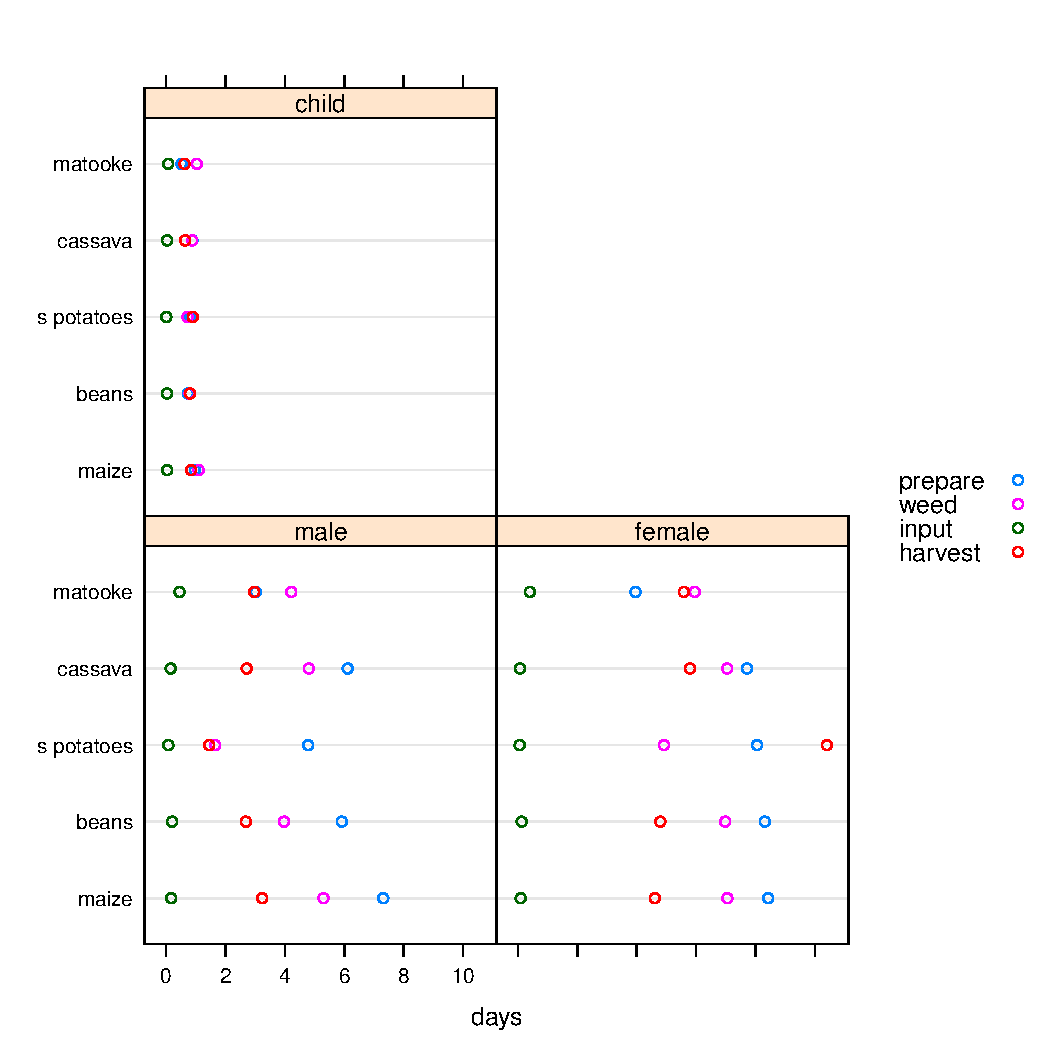
\includegraphics[scale=0.6]{../dotplot}
\end{figure}



\subsubsection*{\newpage{}}


\section*{Appendix}

\begin{table}[H]
\protect\caption{Effect on days worked by mother (full results)\label{tab:appendixmotherh}}
\begin{tabular}{rcccccc} \hline \hline
	&	(1)	&	(2)	&	(3)	&	(4)		&	(5)	

\\
	&	OLS	&	2SLS	&	2SLS	&	2SLS		&	LIML	\\
\hline
	

fgap    &       0.533  &      29.890* &      54.070**  &      40.841** &      38.773** \\             &     (0.735)  &    (17.769)  &    (33.364)  &    (19.353)  &    (19.085)  \\ femhead  &      -7.906* &     -43.577* &     -71.806+ &     -56.883* &     -54.370* \\             &     (3.715)  &    (21.981)  &    (40.831)  &    (24.354)  &    (23.883)  \\ urban    &     -13.317**&     -20.758**&     -25.334* &     -23.534**&     -23.009**\\             &     (3.536)  &     (6.910)  &    (10.247)  &     (8.041)  &     (7.811)  \\ mprim&       0.023  &       4.177  &       3.472  &       5.726  &       5.434  \\             &     (2.754)  &     (4.566)  &     (5.864)  &     (5.194)  &     (5.085)  \\ msec&       1.115  &      -1.624  &       2.608  &      -2.646  &      -2.453  \\             &     (4.706)  &     (5.869)  &     (9.177)  &     (6.913)  &     (6.676)  \\ mthird&     -15.001* &     -46.192* &     -70.087+ &     -57.827* &     -55.630* \\             &     (6.961)  &    (23.251)  &    (38.987)  &    (25.869)  &    (25.530)  \\ health      &      -7.274  &     -11.634+ &      -9.296  &     -13.260  &     -12.953  \\             &     (4.607)  &     (6.967)  &    (11.406)  &     (8.326)  &     (8.044)  \\ school     &       6.740* &       3.705  &       3.073  &       2.573  &       2.786  \\             &     (2.703)  &     (3.837)  &     (6.100)  &     (4.461)  &     (4.334)  \\ cdied     &       6.810+ &       0.209  &      -2.949  &      -2.253  &      -1.788  \\             &     (3.874)  &     (6.592)  &     (9.328)  &     (7.510)  &     (7.333)  \\ cons       &      49.054**&     -10.209  &     -48.668  &     -32.314  &     -28.140  \\             &     (2.815)  &    (36.011)  &    (61.945)  &    (39.017)  &    (38.525)  \\  \\ N           &    2016  &    2016  &    1620  &    2016  &    2016  \\ 
          
instrument:	&	-	&	1st = girl	&	1st \& 2nd = girl	&	\% girl	& 1st = girl \& \% girl	\\ 

\hline \hline 
\multicolumn{6}{l}{\footnotesize Note: Huber-White standard errors in parentheses, +, * and ** denote significance at the 10, 5 and 1 percent}\\
\multicolumn{6}{l}{\footnotesize level respectively.}\\
\end{tabular}
\end{table}


\begin{table}[H]
\protect\caption{Effect on days worked by father (full results)\label{tab:Effect-on-maileappend}}
\begin{tabular}{rcccccc} \hline \hline
	&	(1)	&	(2)	&	(3)	&	(4)		&	(5)	

\\
	&	OLS	&	2SLS	&	2SLS	&	2SLS		&	LIML	\\
\hline
fgap    &      -0.620  &      10.928  &       5.915  &      22.327*  &      20.076+  \\             &     (0.668)  &    (13.983)  &    (25.595)  &    (13.580)  &    (14.756)  \\ femhead  &     -30.349**&     -44.381**&     -39.124  &     -58.231**&     -55.496**\\             &     (2.216)  &    (16.903)  &    (30.436)  &    (16.952)  &    (18.155)  \\ urban    &     -10.103**&     -13.030**&     -14.318**&     -15.919**&     -15.349**\\             &     (2.902)  &     (4.347)  &     (5.249)  &     (5.056)  &     (5.016)  \\ mprim&       1.374  &       3.008  &       2.241  &       4.620  &       4.302  \\             &     (2.717)  &     (3.271)  &     (2.967)  &     (3.769)  &     (3.687)  \\ msec&      -7.239* &      -8.317* &      -9.670* &      -9.381* &      -9.171* \\             &     (3.120)  &     (3.454)  &     (3.770)  &     (4.404)  &     (4.175)  \\ mthird&      -5.829  &     -18.098  &      -9.522  &     -30.209+ &     -27.817  \\             &     (4.926)  &    (16.387)  &    (26.183)  &    (17.049)  &    (17.973)  \\ health      &      -7.849* &      -9.564* &      -9.534* &     -11.257* &     -10.922* \\             &     (3.589)  &     (4.045)  &     (4.444)  &     (5.168)  &     (4.913)  \\ school     &       5.826* &       4.632  &       7.310  &       3.454  &       3.687  \\             &     (2.843)  &     (3.630)  &     (4.782)  &     (3.620)  &     (3.742)  \\ cdied     &       6.756* &       4.159  &       5.314  &       1.596  &       2.102  \\             &     (3.272)  &     (4.374)  &     (5.030)  &     (5.209)  &     (5.089)  \\ cons       &      38.067**&      14.756  &      26.774  &      -8.254  &      -3.711  \\             &     (2.377)  &    (28.289)  &    (47.345)  &    (27.361)  &    (29.750)  \\  \\ N           &    2016  &    2016  &    1620  &    2016  &    2016  \\ 
instrument:	&	-	&	1st = girl	&	1st \& 2nd = girl	&	\% girl	& 1st = girl \& \% girl	\\ 

\hline \hline 
\multicolumn{6}{l}{\footnotesize Note: Huber-White standard errors in parentheses, +, * and ** denote significance at the 10, 5 and 1 percent}\\
\multicolumn{6}{l}{\footnotesize level respectively.}\\
\end{tabular}
\end{table}


\begin{table}
\protect\caption{Effect on days spend on preparing fields (full results)\label{tab:prepappe}}
\begin{tabular}{rcccccc} \hline \hline
	&	(1)	&	(2)	&	(3)	&	(4)		&	(5)	

\\
	&	OLS	&	2SLS	&	2SLS	&	2SLS		&	LIML	\\
\hline
fgap    &      -0.048  &      15.876  &      41.127**  &      26.028** &      25.278* \\             &     (0.528)  &    (12.737)  &    (25.884)  &    (13.720)  &    (14.761)  \\ femhead  &     -15.173**&     -34.568* &     -64.891* &     -46.932**&     -46.018* \\             &     (2.023)  &    (15.704)  &    (31.846)  &    (17.259)  &    (18.412)  \\ urban    &      -6.940**&     -11.013* &     -17.002* &     -13.610* &     -13.418* \\             &     (2.623)  &     (4.481)  &     (7.827)  &     (5.417)  &     (5.493)  \\ mprim 2&      -2.251  &      -0.069  &      -0.597  &       1.322  &       1.219  \\             &     (2.209)  &     (3.307)  &     (4.513)  &     (3.585)  &     (3.703)  \\ msec &      -2.980  &      -4.482  &      -2.924  &      -5.439  &      -5.368  \\             &     (2.832)  &     (3.537)  &     (6.729)  &     (4.377)  &     (4.336)  \\ mthird &     -11.214**&     -28.140+ &     -51.405+ &     -38.931* &     -38.133* \\             &     (3.993)  &    (15.545)  &    (29.529)  &    (17.591)  &    (18.553)  \\ health      &      -3.914  &      -6.215  &      -6.296  &      -7.682  &      -7.573  \\             &     (3.233)  &     (4.293)  &     (8.266)  &     (5.446)  &     (5.379)  \\ school     &       2.919  &       1.343  &       0.511  &       0.338  &       0.412  \\             &     (1.932)  &     (2.546)  &     (4.654)  &     (3.079)  &     (3.073)  \\ cdead     &       5.262+ &       1.632  &      -2.547  &      -0.682  &      -0.511  \\             &     (2.719)  &     (4.291)  &     (7.133)  &     (5.142)  &     (5.203)  \\ cons       &      35.817**&       3.741  &     -39.561  &     -16.708  &     -15.197  \\             &     (2.261)  &    (26.072)  &    (47.770)  &    (27.523)  &    (29.771)   \\ N           &    2015  &    2015  &    1619  &    2015  &    2015  \\ 
instrument:	&	-	&	1st = girl	&	1st \& 2nd = girl	&	\% girl	& 1st = girl \& \% girl	\\ 

\hline \hline 
\multicolumn{6}{l}{\footnotesize Note: Huber-White standard errors in parentheses, +, * and ** denote significance at the 10, 5 and 1 percent}\\
\multicolumn{6}{l}{\footnotesize level respectively.}\\
\end{tabular}
\end{table}


\begin{table}
\protect\caption{Effect on days spend on input application (full results)\label{tab:applappend}}


\begin{tabular}{rcccccc} \hline \hline
	&	(1)	&	(2)	&	(3)	&	(4)		&	(5)	

\\
	&	OLS	&	2SLS	&	2SLS	&	2SLS		&	LIML	\\
\hline
fgap    &       0.051  &       1.812  &       0.849  &       2.372  &       2.224  \\             &     (0.136)  &     (1.632)  &     (1.686)  &     (1.829)  &     (1.741)  \\ femhead  &       0.349  &      -1.795  &      -0.493  &      -2.478  &      -2.297  \\             &     (0.747)  &     (1.611)  &     (1.756)  &     (1.717)  &     (1.628)  \\ urban    &      -0.514  &      -0.964  &      -0.674  &      -1.107  &      -1.069  \\             &     (0.386)  &     (0.713)  &     (0.615)  &     (0.788)  &     (0.763)  \\ mprim &       0.466* &       0.707* &       0.657**&       0.784* &       0.764* \\             &     (0.182)  &     (0.325)  &     (0.246)  &     (0.376)  &     (0.358)  \\ msec &       0.978  &       0.812  &       1.158  &       0.759  &       0.773  \\             &     (0.881)  &     (0.814)  &     (1.126)  &     (0.802)  &     (0.804)  \\ mthird &      -0.684  &      -2.555  &      -1.897  &      -3.151  &      -2.993  \\             &     (1.202)  &     (2.575)  &     (2.550)  &     (2.835)  &     (2.745)  \\ health      &       0.198  &      -0.057  &      -0.088  &      -0.138  &      -0.116  \\             &     (0.489)  &     (0.611)  &     (0.613)  &     (0.687)  &     (0.663)  \\ school     &      -0.045  &      -0.219  &      -0.108  &      -0.275  &      -0.260  \\             &     (0.289)  &     (0.302)  &     (0.339)  &     (0.302)  &     (0.300)  \\ cdead     &      -0.142  &      -0.543  &      -0.235  &      -0.671  &      -0.637  \\             &     (0.222)  &     (0.513)  &     (0.401)  &     (0.591)  &     (0.564)  \\ cons       &       0.526  &      -3.021  &      -0.935  &      -4.150  &      -3.851  \\             &     (0.448)  &     (3.370)  &     (3.238)  &     (3.793)  &     (3.609)   \\ N           &    2015  &    2015  &    1619  &    2015  &    2015  \\ 
instrument:	&	-	&	1st = girl	&	1st \& 2nd = girl	&	\% girl	& 1st = girl \& \% girl	\\ 

\hline \hline 
\multicolumn{6}{l}{\footnotesize Note: Huber-White standard errors in parentheses, +, * and ** denote significance at the 10, 5 and 1 percent}\\
\multicolumn{6}{l}{\footnotesize level respectively.}\\
\end{tabular}
\end{table}


\begin{table}
\protect\caption{Effect on days spend on weeding (full results)\label{tab:timeweeding}}


\begin{tabular}{rcccccc} \hline \hline
	&	(1)	&	(2)	&	(3)	&	(4)		&	(5)	

\\
	&	OLS	&	2SLS	&	2SLS	&	2SLS		&	LIML	\\
\hline

fgap   &       0.026  &      17.708*  &      25.959*  &      21.385* &      20.492* \\             &     (0.468)  &    (11.724)  &    (17.541)  &    (11.730)  &    (11.253)  \\ femhead  &     -13.623**&     -35.158* &     -45.639* &     -39.637**&     -38.550**\\             &     (1.728)  &    (14.648)  &    (21.645)  &    (14.779)  &    (14.180)  \\ urban    &      -9.339**&     -13.862**&     -15.649**&     -14.802**&     -14.574**\\             &     (2.340)  &     (4.495)  &     (5.509)  &     (4.756)  &     (4.613)  \\ mprim &      -0.489  &       1.934  &       1.010  &       2.438  &       2.315  \\             &     (1.772)  &     (2.772)  &     (3.137)  &     (2.968)  &     (2.880)  \\ msec &      -2.274  &      -3.942  &      -2.715  &      -4.289  &      -4.205  \\             &     (2.594)  &     (3.488)  &     (4.834)  &     (3.904)  &     (3.775)  \\ mthird &      -5.350  &     -24.143  &     -30.226  &     -28.052+ &     -27.103+ \\             &     (4.259)  &    (14.960)  &    (20.546)  &    (15.193)  &    (14.766)  \\ health      &      -8.375**&     -10.930**&     -10.259+ &     -11.461**&     -11.332**\\             &     (2.059)  &     (3.844)  &     (5.363)  &     (4.270)  &     (4.136)  \\ school     &       4.598**&       2.848  &       3.290  &       2.484  &       2.572  \\             &     (1.751)  &     (2.336)  &     (3.165)  &     (2.470)  &     (2.417)  \\ cdead     &       5.040* &       1.010  &       0.656  &       0.172  &       0.375  \\             &     (2.323)  &     (4.315)  &     (5.183)  &     (4.525)  &     (4.412)  \\ cons       &      29.534**&      -6.083  &     -17.387  &     -13.490  &     -11.692  \\             &     (1.783)  &    (23.464)  &    (32.493)  &    (23.516)  &    (22.524)    \\ N           &    2015  &    2015  &    1619  &    2015  &    2015  \\ 
instrument:	&	-	&	1st = girl	&	1st \& 2nd = girl	&	\% girl	& 1st = girl \& \% girl	\\ 

\hline \hline 
\multicolumn{6}{l}{\footnotesize Note: Huber-White standard errors in parentheses, +, * and ** denote significance at the 10, 5 and 1 percent}\\
\multicolumn{6}{l}{\footnotesize level respectively.}\\
\end{tabular}
\end{table}


\begin{table}
\protect\caption{Effect on days spend on harvesting (full results)}
\begin{tabular}{rcccccc} \hline \hline
	&	(1)	&	(2)	&	(3)	&	(4)		&	(5)	

\\
	&	OLS	&	2SLS	&	2SLS	&	2SLS		&	LIML	\\
\hline

fgap    &      -0.082  &       5.315  &      -3.591  &      13.852+  &      12.485+  \\             &     (0.468)  &    (10.597)  &    (20.563)  &     (8.987)  &    (10.379)  \\ femhead  &     -10.650**&     -17.223  &      -6.270  &     -27.620* &     -25.955* \\             &     (1.771)  &    (12.609)  &    (24.287)  &    (11.128)  &    (12.624)  \\ urban    &      -6.876**&      -8.257**&      -8.124* &     -10.440**&     -10.091**\\             &     (1.873)  &     (2.977)  &     (3.852)  &     (3.362)  &     (3.402)  \\ mprim &       2.741  &       3.481  &       3.569+ &       4.650+ &       4.463+ \\             &     (1.906)  &     (2.131)  &     (2.042)  &     (2.511)  &     (2.448)  \\ msec &      -1.835  &      -2.344  &      -2.761  &      -3.149  &      -3.020  \\             &     (2.343)  &     (2.335)  &     (2.849)  &     (2.969)  &     (2.822)  \\ mthird &      -3.720  &      -9.457  &      -0.912  &     -18.530+ &     -17.078  \\             &     (3.366)  &    (11.938)  &    (20.598)  &    (11.097)  &    (12.290)  \\ health      &      -2.340  &      -3.120  &      -0.215  &      -4.353  &      -4.156  \\             &     (3.167)  &     (3.283)  &     (4.032)  &     (4.004)  &     (3.853)  \\ school     &       5.394* &       4.860+ &       6.889+ &       4.015  &       4.150  \\             &     (2.150)  &     (2.803)  &     (3.685)  &     (2.604)  &     (2.760)  \\ cdead     &       3.501  &       2.271  &       3.443  &       0.325  &       0.637  \\             &     (2.351)  &     (2.914)  &     (3.565)  &     (3.384)  &     (3.345)  \\ cons       &      22.551**&      11.680  &      29.707  &      -5.516  &      -2.763  \\             &     (1.469)  &    (21.379)  &    (38.106)  &    (18.133)  &    (20.921)   \\ N           &    2015  &    2015  &    1619  &    2015  &    2015  \\ 
instrument:	&	-	&	1st = girl	&	1st \& 2nd = girl	&	\% girl	& 1st = girl \& \% girl	\\ 

\hline \hline 
\multicolumn{6}{l}{\footnotesize Note: Huber-White standard errors in parentheses, +, * and ** denote significance at the 10, 5 and 1 percent}\\
\multicolumn{6}{l}{\footnotesize level respectively.}\\
\end{tabular}
\end{table}


\begin{table}
\protect\caption{Total production (full tobit results)}


\begin{tabular}{rcccccc} \hline \hline
	&	(1)	&	(2)	&	(3)	&	(4)		&	(5)	

\\
	&	OLS	&	2SLS	&	2SLS	&	2SLS		&	LIML	\\
\hline

fgap    &      -3.411  &      21.056  &     -20.275  &      16.988  &      19.334  \\             &     (2.697)  &    (46.911)  &    (57.977)  &    (48.493)  &    (44.172)  \\ femhead  &     -69.276**&     -97.608+ &     -41.725  &     -92.870  &     -95.599+ \\             &    (13.700)  &    (55.994)  &    (67.508)  &    (57.696)  &    (52.888)  \\ urban    &    -191.662**&    -199.111**&    -183.271**&    -197.891**&    -198.597**\\             &    (13.527)  &    (18.843)  &    (19.978)  &    (19.209)  &    (18.219)  \\ mprim &      31.542**&      35.247**&      40.222**&      34.604**&      34.970**\\             &     (9.652)  &    (12.321)  &    (11.070)  &    (12.382)  &    (12.050)  \\ msec &     -14.660  &     -20.572  &     -17.281  &     -19.563  &     -20.150  \\             &    (14.527)  &    (17.768)  &    (20.052)  &    (17.924)  &    (17.324)  \\ mthird &      29.624  &       2.888  &      78.249  &       7.286  &       4.749  \\             &    (35.753)  &    (58.152)  &    (63.402)  &    (59.720)  &    (55.538)  \\ health      &     -12.603  &     -15.259  &     -10.523  &     -14.869  &     -15.089  \\             &    (15.952)  &    (16.802)  &    (19.526)  &    (16.816)  &    (16.688)  \\ school     &      37.105**&      36.348**&      39.394**&      36.483**&      36.411**\\             &     (9.238)  &     (9.316)  &    (10.397)  &     (9.273)  &     (9.279)  \\ cdied     &      15.566  &       8.472  &       9.039  &       9.642  &       8.970  \\             &    (12.878)  &    (18.682)  &    (18.569)  &    (18.990)  &    (18.093)  \\  cons       &     153.527**&     100.065  &     197.728  &     108.964  &     103.831  \\             &    (12.388)  &   (103.164)  &   (121.588)  &   (106.568)  &    (97.211)  \\  \\
N           &    2637  &    2637  &    2020  &    2637  &    2637  \\


instrument:	&	-	&	1st = girl	&	1st \& 2nd = girl	&	\% girl	& 1st = girl \& \% girl	\\ 

\hline \hline 
\multicolumn{6}{l}{\footnotesize Note: Huber-White standard errors in parentheses, +, * and ** denote significance at the 10, 5 and 1 percent}\\
\multicolumn{6}{l}{\footnotesize level respectively.}\\
\end{tabular}
\end{table}


\begin{table}
\protect\caption{Total production per capita (full tobit results)}


\begin{tabular}{rcccccc} \hline \hline
	&	(1)	&	(2)	&	(3)	&	(4)		&	(5)	

\\
	&	OLS	&	2SLS	&	2SLS	&	2SLS		&	LIML	\\
\hline

fgap    &       4.133**&      10.501  &      -9.251  &      14.517  &      12.340  \\             &     (1.527)  &    (26.009)  &    (24.107)  &    (27.183)  &    (24.605)  \\ femhead  &     -39.851**&     -47.223  &     -10.658  &     -51.859  &     -49.346+ \\             &     (7.938)  &    (31.039)  &    (28.068)  &    (32.335)  &    (29.453)  \\ substrat    &     -98.207**&    -100.147**&     -67.933**&    -101.377**&    -100.709**\\             &     (8.560)  &    (10.451)  &     (8.290)  &    (10.764)  &    (10.150)  \\ mprim &      20.087**&      21.052**&      17.671**&      21.646**&      21.324**\\             &     (5.220)  &     (6.835)  &     (4.606)  &     (6.946)  &     (6.716)  \\ msec &      -3.727  &      -5.265  &      -4.161  &      -6.221  &      -5.707  \\             &     (8.632)  &     (9.846)  &     (8.330)  &    (10.040)  &     (9.644)  \\ mthird &      20.268  &      13.311  &      55.245* &       8.899  &      11.294  \\             &    (24.284)  &    (32.189)  &    (26.298)  &    (33.422)  &    (30.880)  \\ health      &      -8.756  &      -9.447  &      -8.607  &      -9.909  &      -9.653  \\             &     (8.925)  &     (9.326)  &     (8.131)  &     (9.440)  &     (9.308)  \\ school     &      12.227* &      12.030* &      11.697**&      11.910* &      11.976* \\             &     (4.969)  &     (5.167)  &     (4.325)  &     (5.203)  &     (5.172)  \\ cdied     &       5.932  &       4.085  &       2.685  &       2.916  &       3.551  \\             &     (7.121)  &    (10.360)  &     (7.726)  &    (10.649)  &    (10.082)  \\  cons       &      49.910**&      35.996  &      68.721  &      27.226  &      31.979  \\             &     (6.365)  &    (57.199)  &    (50.558)  &    (59.739)  &    (54.151)  \\ \\
N           &    2637  &    2637  &    2020  &    2637  &    2637  \\ 

instrument:	&	-	&	1st = girl	&	1st \& 2nd = girl	&	\% girl	& 1st = girl \& \% girl	\\ 

\hline \hline 
\multicolumn{6}{l}{\footnotesize Note: Huber-White standard errors in parentheses, +, * and ** denote significance at the 10, 5 and 1 percent}\\
\multicolumn{6}{l}{\footnotesize level respectively.}\\
\end{tabular}
\end{table}


\begin{table}
\protect\caption{Total area (full tobit results)}


\begin{tabular}{rcccccc} \hline \hline
	&	(1)	&	(2)	&	(3)	&	(4)		&	(5)	

\\
	&	OLS	&	2SLS	&	2SLS	&	2SLS		&	LIML	\\
\hline

fgap    &      -0.033  &       0.120  &       0.042  &       0.145  &       0.132  \\             &     (0.023)  &     (0.343)  &     (0.443)  &     (0.359)  &     (0.325)  \\ femhead  &      -0.511**&      -0.689+ &      -0.530  &      -0.718+ &      -0.703+ \\             &     (0.097)  &     (0.410)  &     (0.516)  &     (0.427)  &     (0.389)  \\ urban    &      -1.351**&      -1.398**&      -1.345**&      -1.406**&      -1.401**\\             &     (0.111)  &     (0.138)  &     (0.153)  &     (0.142)  &     (0.134)  \\ mprim &       0.172* &       0.196* &       0.250**&       0.199* &       0.197*   \\             &     (0.071)  &     (0.090)  &     (0.085)  &     (0.091)  &     (0.089)  \\ msec &      -0.175  &      -0.212  &      -0.215  &      -0.218  &      -0.215+   \\             &     (0.111)  &     (0.130)  &     (0.153)  &     (0.133)  &     (0.127)  \\ mthird &      -0.035  &      -0.202  &       0.088  &      -0.230  &      -0.215    \\             &     (0.210)  &     (0.428)  &     (0.487)  &     (0.443)  &     (0.411)  \\ health      &      -0.133  &      -0.150  &      -0.158  &      -0.153  &      -0.151  \\             &     (0.108)  &     (0.123)  &     (0.150)  &     (0.125)  &     (0.123)  \\ school     &       0.310**&       0.306**&       0.331**&       0.305**&       0.305**\\             &     (0.070)  &     (0.068)  &     (0.080)  &     (0.069)  &     (0.068)  \\ cdied     &       0.103  &       0.058  &       0.012  &       0.051  &       0.055  \\             &     (0.093)  &     (0.137)  &     (0.142)  &     (0.140)  &     (0.133)   \\ cons       &       0.793**&       0.459  &       0.630  &       0.403  &       0.432  \\             &     (0.080)  &     (0.755)  &     (0.930)  &     (0.788)  &     (0.715)  \\  \\
N           &    2637  &    2637  &    2020  &    2637  &    2637  \\
instrument:	&	-	&	1st = girl	&	1st \& 2nd = girl	&	\% girl	& 1st = girl \& \% girl	\\ 

\hline \hline 
\multicolumn{6}{l}{\footnotesize Note: Huber-White standard errors in parentheses, +, * and ** denote significance at the 10, 5 and 1 percent}\\
\multicolumn{6}{l}{\footnotesize level respectively.}\\
\end{tabular}
\end{table}


\begin{table}
\protect\caption{Total yield (x1000 UGX per acre)}
\begin{tabular}{rcccccc} \hline \hline
	&	(1)	&	(2)	&	(3)	&	(4)		&	(5)	

\\
	&	OLS	&	2SLS	&	2SLS	&	2SLS		&	LIML	\\
\hline

fgap    &      -1.697  &      43.088  &     -96.861  &       0.013  &       8.818  \\             &     (2.862)  &    (81.451)  &   (140.870)  &    (61.118)  &    (69.674)  \\ femhead  &     -32.827* &     -82.434  &      62.869  &     -34.721  &     -44.474  \\             &    (13.620)  &    (91.141)  &   (149.672)  &    (69.314)  &    (78.576)  \\ urban    &     -19.120  &     -31.562  &     -17.771  &     -19.596  &     -22.042  \\             &    (17.498)  &    (29.340)  &    (36.155)  &    (24.900)  &    (26.586)  \\ mprim &       9.668  &      12.719  &      17.577  &       9.785  &      10.384   \\             &    (11.889)  &    (14.153)  &    (21.954)  &    (12.962)  &    (13.267)  \\ msec &      34.954+ &      32.322  &      24.785  &      34.854+ &      34.336+   \\             &    (20.106)  &    (22.005)  &    (27.654)  &    (20.229)  &    (20.478)  \\ mthird &      11.594  &     -41.631  &     115.467  &       9.562  &      -0.903    \\             &    (38.115)  &    (99.945)  &   (156.775)  &    (78.774)  &    (87.257)  \\ health      &      -9.314  &     -18.619  &       0.558  &      -9.669  &     -11.498  \\             &    (17.760)  &    (26.018)  &    (27.844)  &    (21.578)  &    (22.827)  \\ school     &      10.851  &       5.932  &      28.583  &      10.663  &       9.696  \\             &    (11.524)  &    (15.622)  &    (23.309)  &    (13.193)  &    (13.852)  \\ cdied     &       1.373  &     -14.487  &      22.702  &       0.767  &      -2.351  \\             &    (16.065)  &    (30.019)  &    (38.702)  &    (25.321)  &    (27.246)  \\ 
cons       &     178.153**&     154.719  &     449.143  &     244.882+ &     226.452  \\             &    (16.668)  &   (171.814)  &   (283.600)  &   (130.707)  &   (148.357)  \\ \\ 
N           &    1567  &    1567  &    1278  &    1567  &    1567  \\

instrument:	&	-	&	1st = girl	&	1st \& 2nd = girl	&	\% girl	& 1st = girl \& \% girl	\\ 

\hline \hline 
\multicolumn{6}{l}{\footnotesize Note: Huber-White standard errors in parentheses, +, * and ** denote significance at the 10, 5 and 1 percent}\\
\multicolumn{6}{l}{\footnotesize level respectively.}\\
\end{tabular}
\end{table}

\end{document}
